\section{Design}
\label{sec:design}

\subsection{Model overview}
I constructed a Markov state-transition model to compare lifetime outcomes for two hypothetical cohorts of otherwise identical individuals: one cohort that donates a kidney and one that does not. Both cohorts enter the model at the age of donation in full health, and the simulation advances in annual cycles until age~110. The analysis was conducted from the perspective of the individual donor rather than the health-care system; outcomes are reported as undiscounted remaining life-years, consistent with the standard approach for life-expectancy analyses.~\cite{gold_cost_1996} The base-case age at donation is 40 years; subgroup analyses span ages 25--55. I used a Monte Carlo simulation with $5 \times 10^6$ individuals per arm and cross-validated against a deterministic analytic cohort implementation. I used annual (one-year) cycles throughout. 
% Life-years accumulated with an end-of-cycle convention; the resulting systematic underestimate of approximately 0.5~years applies equally to both arms and cancels in $\Delta$LE. 
I did not discount future life-years, consistent with the convention for pure life-expectancy analyses.~\cite{gold_cost_1996}

\begin{figure}
	\centering
	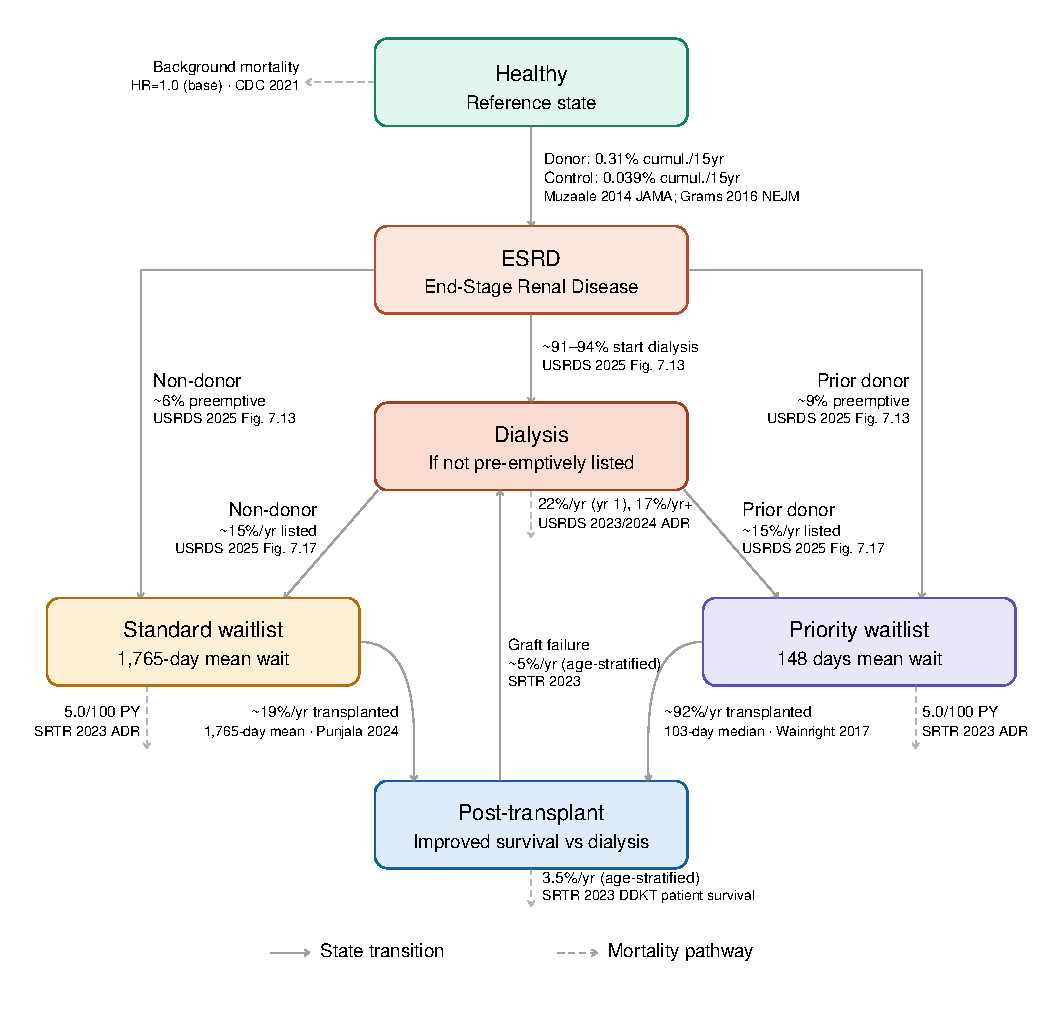
\includegraphics[width=\linewidth]{figures/markov_model_kidney_donation.pdf}
	\caption{The Markov model for kidney donation.}
	\label{fig:markov}
\end{figure}

\subsection{Health states}
The model contains seven mutually exclusive health states (Figure~\ref{fig:markov}): \textit{Healthy}, \textit{ESRD onset}, \textit{Dialysis}, \textit{Standard waitlist}, \textit{Priority waitlist}, \textit{Post-transplant}, and \textit{Dead} (absorbing). At ESRD onset, the cohort branches: a fraction is listed preemptively (bypassing dialysis entirely) and the remainder initiates haemodialysis. The donor arm routes ESRD survivors to the \textit{Priority waitlist}, reflecting the allocation priority afforded to prior living donors (PLD) under KAS250; the non-donor arm routes to the \textit{Standard waitlist}. Graft failure returns patients to the \textit{Dialysis} state, bypassing the ESRD-onset branch.

\subsection{ESRD risk after donation}
Fifteen-year cumulative ESRD incidence was taken from Muzaale et al.~\cite{muzaale_risk_2014}: 30.8 per 10,000 (95\%~CI 24.3--38.5) for donors and 3.9 per 10,000 (95\%~CI 0.8--8.9) for age-, sex-, and health-matched controls (8-fold relative risk). Race-specific donor rates were 74.7/10,000 (Black) and 22.7/10,000 (White).~\cite{muzaale_risk_2014} The White non-donor baseline was taken from Grams et al.~\cite{grams_kidney-failure_2016} (sex-averaged 0.05\%/15~yr), because zero ESRD events were recorded in White matched controls in Muzaale et al.

I modelled ESRD hazard with a Weibull distribution (shape $k = 1.5$), calibrated via a competing-risk bisection algorithm to reproduce the 15-year cumulative incidence while accounting for background-mortality attrition in the at-risk pool. The accelerating hazard ($k > 1$) is supported by the Massie et al.\ 20-year cumulative incidence of 34 per 10,000 (vs.\ $\approx$21/10,000 predicted under a constant-hazard model).~\cite{massie_quantifying_2017} I drew within-donor subgroup hazard ratios from Massie et al.: 2.96 (95\%~CI 2.25--3.89) for Black race, 1.88 (95\%~CI 1.50--2.35) for male sex, and 1.40 per decade (non-Black donors).~\cite{massie_quantifying_2017}

\subsection{Dialysis survival and waitlist listing}
First-year haemodialysis mortality was 22\% and subsequent-year mortality 17\% ($\approx$42\% five-year survival), consistent with USRDS estimates.~\cite{usrds_2024}

At ESRD onset, a fraction of patients is listed preemptively before dialysis initiation, avoiding dialysis mortality entirely. I drew preemptive listing probabilities from USRDS 2025 ADR Figure~7.13: 5.8\% overall for the non-donor arm and 9.4\% for the donor arm (age 18--44 cohort, reflecting the younger and healthier donor-like population).~\cite{usrds_2025}

Among patients on dialysis, the conditional annual probability of joining the waitlist was set to 15\%/year (base case), derived from USRDS 2025 ADR
Figure~7.17.~\cite{usrds_2025} Approximately 25\% of 18--44 year-old ESRD patients are listed or transplanted within one year, of whom $\approx$9.4\% were preemptively listed, yielding an estimated post-dialysis listing rate of $\approx$15.6\%/year for the donor-like cohort (conservative base case: 15\%/year; one-way sensitivity range 5--30\%/year).

\subsection{Transplant waiting time and waitlist outcomes}
Transplant probability while listed was modelled as a time-homogeneous exponential process parameterised by the median waiting time, a standard approximation for waiting-time analyses.~\cite{krahn_primer_1997} For the standard waitlist, I used the post-KAS250 national median of 985~days;~\cite{schold_effect_2023} for the PLD priority waitlist, I used the post-KAS median of 102.6~days was used.~\cite{wainright_impact_2017} Waitlist mortality was 5.0 deaths per 100 patient-years (SRTR 2023 ADR Figure~KI~24) and competing removal 6.81\%/year (SRTR 2023 ADR
Figure~KI~22).~\cite{srtr_2023}

\subsection{Post-transplant survival}
I derived post-transplant annual mortality from age-stratified 5-year Kaplan--Meier estimates for DDKT recipients in the SRTR 2023 ADR (Figure~KI~70, 2016--2018 cohort): 0.9\%/year (ages 18--34), 1.8\%/year (35--49), 3.9\%/year (50--64), and 6.9\%/year ($\geq 65$).~\cite{srtr_2023} The base case uses DDKT survival because prior living donors who develop ESRD predominantly receive transplants via the deceased-donor priority pathway rather than living-donor transplantation, consistent with USRDS data showing that living-donor transplants account for a small minority of transplants in this population.~\cite{brar2018mortality,muzaale2016recipient} A one-way sensitivity analysis substitutes LDKT patient survival (SRTR 2023 ADR Figure~KI~76: 0.4\%, 0.8\%, 1.7\%, and 3.9\%/year by age band) to bound the effect of this assumption. Annual graft failure was 2.5\%/year post-year~1;~\cite{srtr_2023} graft failure returned patients to the Dialysis state.

\subsection{Background mortality and donor all-cause survival}
I took background mortality in the Healthy state from the 2021 US Life Tables (CDC, National Vital Statistics Reports Vol.~72 No.~12),~\cite{cdc_2023} with sex-specific tables used in sex-stratified analyses. The base-case donor all-cause mortality hazard ratio versus matched non-donors is 1.0, consistent with US-based studies~\cite{muzaale_risk_2014,segev_perioperative_2010} and the Grams et al.\ 2018 meta-analysis (pooled HR 0.984, 95\%~CI 0.743--1.302; 9 studies, $n = 118{,}426$ donors).~\cite{grams_mid-_2018} I also examined an HR of 1.30 from Mjøen et al.\ \cite{mjoeen_long-term_2014}, derived from a Norwegian cohort in which 80\% of donors were first-degree relatives of the recipient, as the pessimistic sensitivity scenario.

\subsection{Subgroup analyses}

\subsubsection{Age at donation}
I repeated the analyses at ages 25, 35, 40, 45, and 55~years at donation. Donor ESRD rates were scaled by the Massie~2017 age HR (1.40/decade, non-Black donors);~\cite{massie_quantifying_2017} I held non-donor baselines at the Muzaale overall matched-control rate.

\subsubsection{Race}
I took race-specific donor ESRD rates (Black 74.7/10,000; White 22.7/10,000) and race-specific non-donor baselines (Black sex-averaged 0.195\%/15~yr; White sex-averaged 0.05\%/15~yr) from Muzaale et al.\ \cite{muzaale_risk_2014} and Grams et al., respectively.~\cite{grams_kidney-failure_2016} Race-specific waitlist mortality and post-transplant survival were from SRTR 2023 Figures~KI~25 and KI~71.~\cite{srtr_2023}

\subsubsection{Sex}
I derived sex-specific donor ESRD rates were derived by applying the Massie~2017 male-sex HR (1.88)~\cite{massie_quantifying_2017} to the overall donor rate, weighted by the observed donor sex mix (60\% female; SRTR 2023 ADR Figure~KI~7).~\cite{srtr_2023} For non-donor baselines, we used the Grams~2016 White sex-specific rates (female 0.04\%/15~yr; male 0.06\%/15~yr) rather than applying the within-donor sex HR to the control arm, because Massie~2017 hazard ratios describe variation within the donor cohort and are not appropriate for scaling a different reference population.~\cite{grams_kidney-failure_2016} I applied this sourcing rule, Muzaale matched-control rates for overall analyses and Grams direct rates wherever sex or race is stratified, consistently across all simulations.

\subsection{Probabilistic sensitivity analysis}
I conducted a PSA with 200 parameter draws. Sampled quantities and their distributions were:
\begin{itemize}
	\item ESRD 15-year cumulative risks: beta distributions parameterised from the Muzaale~2014 published 95\%~CIs;
	\item Donor all-cause mortality HR: log-normal, $\mu = {-0.016}$, $\sigma = 0.143$, derived from the Grams~2018 meta-analysis CI;
	\item Weibull shape $k$: log-normal, $\sigma = 0.13$, representing structural uncertainty absent published CIs for this parameter; and
	\item Waitlist listing probability: beta, fractional SE~=~40\%, consistent with the 0.05--0.30 plausible range
\end{itemize}
Registry-derived parameters (from SRTR or USRDS) have negligible sampling error relative to structural uncertainty and were fixed at base-case values; scenario variation in these parameters is captured by the one-way sensitivity analysis. I report the mean $\Delta$LE, 95\%~credible interval, and the probability that donation is life-expectancy--neutral or beneficial.

\subsection{One-way sensitivity analysis}
I varied each parameter individually:
\begin{itemize}
	\item No priority access and changing the PLD wait time
	\item Donor all-cause mortality HR~=~1.30 from the Mjøen pessimistic estimate
	\item ESRD relative risk from the Mjøen upper-bound on ESRD HR
	\item Post-transplant survival at LDKT quality
	\item Dialysis mortality~$\pm 50\%$
\end{itemize}

\subsection{Calibration}
I validated the model's transplant probability against the SRTR 2023 3-year waitlist outcome distribution (Figure~KI~22, 2019--2021 listing cohort).~\cite{srtr_2023} This comparison is non-circular because I derived the transplant probability from the median waiting time, not from the 3-year outcome distribution. The model predicted 44.3\% transplanted at three years versus 44.3\% observed (DDKT + LDKT combined; $\Delta = 0\%$). I back-calculated the waitlist removal rate via a competing-risk bisection algorithm to reproduce the SRTR-observed 19.1\% removed at three years (12.6\%/year); the na\"{i}ve formula $1-(1-\mathrm{CIF})^{1/3}$, which ignores competing depletion by transplantation and death, was not used. The model over-predicted three-year waitlist mortality (10.0\% vs.\ 6.8\% observed, $\Delta = +47\%$), likely reflecting the application of a 2023 cross-sectional mortality rate (confirmed 5.0/100 patient-years from the raw SRTR data file) to a 2019--2021 listing cohort; this bias is symmetric across both arms and conservative (slightly overstates the cost of the waitlist period for both donors and non-donors equally). No independent cohort exists tracing the complete pathway from living donation through ESRD onset to transplantation; this check represents the available face-validity evidence for the model.

\subsection{Voucher benefit}
\label{sec:methods-voucher}
A kidney-donation ``voucher'' is a mechanism by which a living donor designates a healthy, non-donor family member to receive PLD priority-waitlist access should that family member ever develop ESRD. I simulated two arms of healthy non-donors, both carrying non-donor baseline ESRD risk and a background all-cause mortality HR of 1.0; the sole difference between arms was waitlist priority upon ESRD onset (voucher arm: PLD median wait 102.6~days~\cite{wainright_impact_2017}; control arm: standard median wait 985~days~\cite{schold_effect_2023}). Consistent with the sourcing rule used for the base-case preemptive-listing parameters, I assigned the voucher arm the informed/monitored preemptive-listing probability (9.4\%) and the control arm the general-population probability (5.8\%).~\cite{usrds_2025} All other transition probabilities (dialysis mortality, per-cycle waitlist listing, waitlist mortality and removal, post-transplant survival, graft failure) were identical to the base-case model. I ran the analysis at the base-case age of 40 with an age sweep (25--60~years) and an ESRD-risk subgroup analysis using the Muzaale overall and Grams race-specific non-donor CIFs.~\cite{muzaale_risk_2014,grams_kidney-failure_2016} One-way sensitivity analyses varied the voucher and standard median wait times, the per-cycle listing probability, the preemptive-listing probability, and post-transplant graft quality (DDKT vs.\ LDKT).

\subsection{ESRD-conditional priority benefit}
\label{sec:methods-esrd}
Because the voucher (and, by extension, the donor PLD-priority) benefit is diluted at the population level by the large fraction of the cohort who never develop ESRD, I ran a second model conditioned entirely on ESRD onset. All individuals entered the model already diagnosed with ESRD in order to isolate the life-expectancy benefit of priority waitlist access for the sub-population who actually reach the waitlist. Entry to dialysis versus preemptive listing, dialysis and waitlist mortality, waitlist removal, post-transplant survival, and graft failure used the same age-stratified, all-cause parameters as the base-case model; no separate Healthy state or background-mortality term was included, since dialysis- and waitlist-state mortality rates are all-cause rates already measured in ESRD populations. I compared two arms, differing only in waitlist priority (priority vs.\ standard median wait, as above). The base case used an ESRD-onset age of 60 with an age sweep (40--75~years at ESRD onset) and one-way sensitivity analyses on wait times, per-cycle listing probability, preemptive-listing probability, post-transplant graft quality, and dialysis mortality ($\pm$20\%).

\subsection{Software and reproducibility}
I implemented All analyses in Python~3.10 (NumPy, pandas, matplotlib). The simulation, parameter assembly pipeline, sensitivity analyses, and calibration checks are fully reproducible from the public code repository at \url{https://github.com/rupumped/kidney-donor-le}.